\subsection{Ejercicio 10}
  \begin{figure}
  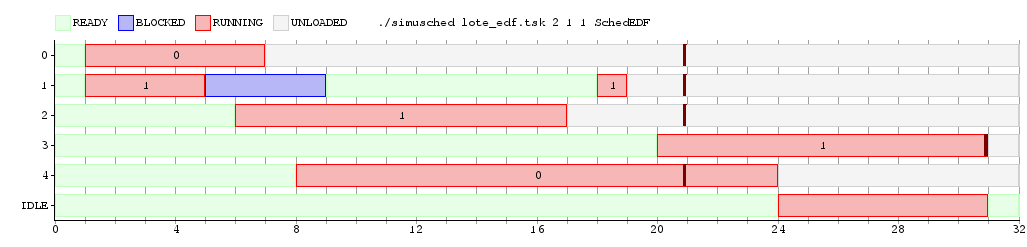
\includegraphics[scale=0.32]{images/lote.png}
  \caption{Scheduler EDF en 2 cores}
  \end{figure}
  \begin{figure}
  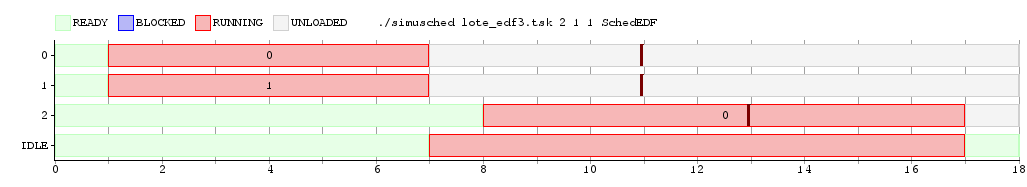
\includegraphics[scale=0.32]{images/lote3.png}
  \caption{Scheduler EDF en 2 cores}
  \end{figure}
La propiedad del edf en estos casos (figuras 14 a 15) no se mantiene, porque aunque la suma de las tareas y sus deadlines es menor a 2, el scheduler es incapaz de hacer que se cumpla la tarea 3, aun cuando la propiedad del edf debiera ser valida.
Para mantener la propiedad de que se cumplan los deadline en un scheduler multicore, se debería usar otro algoritmo que tenga en cuenta como maximizar el uso de los procesadores, ya que para el caso de lote\_edf3.tsk, si el primer core hubiera corrido las 2 tareas de 5 y el segundo hubiese corrido la de 8, todas las tareas se habrían podido lograr en el tiempo necesario.